\documentclass[12pt]{amsart}
\usepackage{geometry}
\geometry{letterpaper}
\usepackage[parfill]{parskip}
\usepackage{graphicx}
\usepackage{amssymb}
\usepackage{epstopdf}
\usepackage{listings}
\DeclareGraphicsRule{.tif}{png}{.png}{`convert #1 `dirname #1`/`basename #1 .tif`.png}

\title{Final Report: The Lorenz Model}
\author{Phil Mayer}

\begin{document}
\maketitle

\section{Background}
For my final project, I chose to explore the Lorenz model, known otherwise as the Lorenz equations. Originally introduced by Edward Norton 
Lorenz, a pioneer in the study of chaos, the model's three equations were originally a simplification of the Navier-Stokes equations, made
because of the weaker computing power back in the 1960's. Despite oversimplifying the Navier-Stokes equations, Lorenz discovered a system 
with rich dynamics and chaotic behavior, given certain combinations of the initial conditions and system parameters. I chose to study this topic
because the Lorenz attractor is one of the most visually recognizable chaotic models, and I recognized its image in the textbook, which I was
able to duplicate as I will show shortly.

Though the problem was originally studied in the context of weather and fluid mechanics, the Lorenz model can be used to describe a wide
variety of physical systems. Its three equations use three parameters: $\sigma, r, b > 0$. Though these are occasionally given physical meaning,
it is best to continue generally. The system's three differential equations using these parameters are:
\begin{align*}
	\frac{dx}{dt} &= \sigma(y - x) \\
	\frac{dy}{dt} &= -xz + rx - y \\
	\frac{dz}{dt} &= xy - bz
\end{align*}
While we can explore the behavior of the system with any positive values of $\sigma, r,$ and $b$, most physicists and mathematicians who
have explored the Lorenz model use $\sigma = 10$ and $b = \frac{8}{3} \approx 2.6667$. Given this convention, the system appears
deceptively simple; it proves to have considerably complex behavior regardless by just modifying $r$ and the initial conditions $x_0, y_0, z_0$.

\newpage
\section{Numerical Methods}
In order to solve the three differential equations numerically, we can apply the Euler method to the each equation, approximating $x, y,$ and $z$
at a range of times. Working up from the initial values $x_0, y_0, z_0$, some time step size $\Delta t$, and a number of points $n$, we can
calculate $x_i, y_i, z_i$ from $i = 1$ to $i = n - 1$ as:
\begin{align*}
	x_i &= x_{i-1} + \frac{dx}{dt} \Delta t \\
	y_i &= y_{i-1} + \frac{dy}{dt} \Delta t \\
	z_i &= z_{i-1} + \frac{dz}{dt} \Delta t
\end{align*}
We can then apply the definitions of $\frac{dx}{dt}, \frac{dy}{dt}, \frac{dz}{dt}$ as described in the previous section to arrive at:
\begin{align*}
	x_i &=  x_{i-1} + \sigma(y_{i-1} - x_{i-1}) \Delta t \\
	y_i &= y_{i-1} + (-x_{i-1}z_{i-1} + rx_{i-1} - y_{i-1}) \Delta t \\
	z_i &= z_{i-1} + (x_{i-1}y_{i-1} - bz_{i-1}) \Delta t
\end{align*}
We can derive this solution by recalling that for some arbitrary number of points $n$ and points $x_i$ (over indices $1 \leq i \leq n - 1$), we can
estimate $\frac{dx}{dt}$ using backward differencing:
\[
	\frac{dx}{dt} \approx \frac{x_i - x_{i - 1}}{\Delta t}
\]
\newline
With only a few steps of simple algebraic manipulation, we arrive at the Euler method.
\[
	x_i \approx x_{i-1} + \frac{dx}{dt} \Delta t
\]
We then apply this to solve the differential equations $\frac{dy}{dt}$ and $\frac{dz}{dt}$ for $y$ and $z$ similarly, then plug in the appropriate
definitions of $\frac{dy}{dt}$ and $\frac{dz}{dt}$ based on the Lorenz model. In this particular problem, the Euler-Cromer method does not
suit our application, since we have three first-order ODEs (whereas the Euler-Cromer method is used to solve second-order ODEs). As the book
describes, some of the factors in the Lorenz model also serve the same purpose as the damping term and the driving force in the case
of the pendulum; given small enough values of $\Delta t$, the associated errors contributed by these terms will tend to cancel, eliminating the
need to use methods like Euler-Cromer. As we will see shortly in the investigation of stability, this can cause some interesting behaviors when
graphing the system.

\newpage
\section{Results}
Overall, I had success reproducing the graphics in the book using my program. For example, the following graph was generated using 
$N = 50,000$, $\Delta t = 0.001$, $\sigma = 10.0$, $b = 2.6667$, $r = 25.0$, and initial conditions $x_0 = 1.0$, $y_0 = z_0 = 0.0$, and has the 
expected appearance of the Lorenz attractor.
\begin{figure}[h]
	\begin{center}
		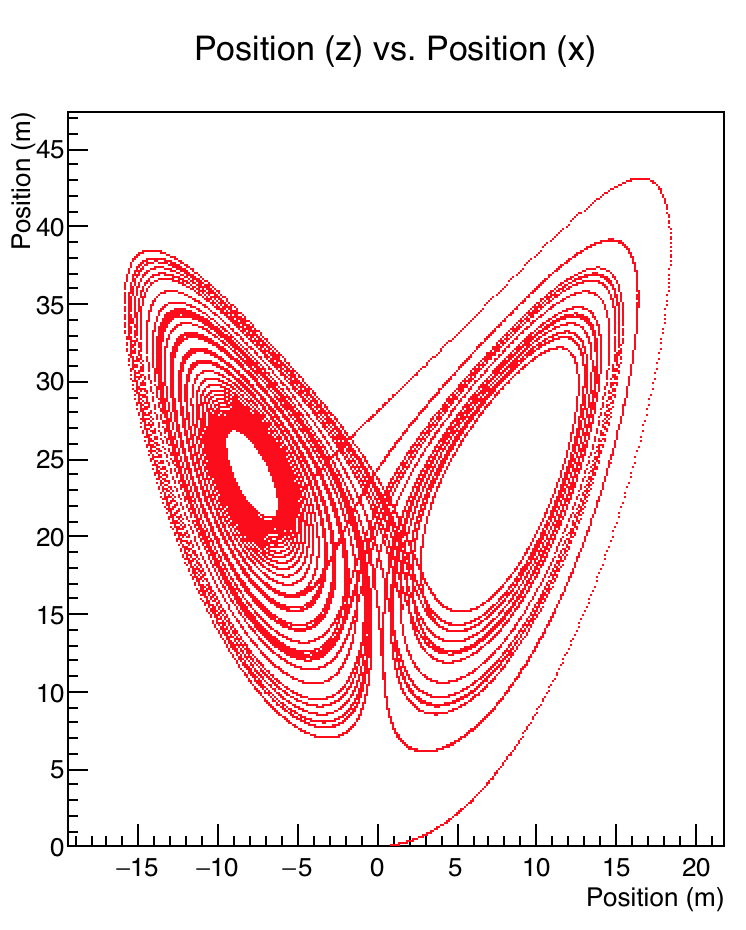
\includegraphics[scale=0.65]{fig-1.png}
	\end{center}
	\caption{The Lorenz attractor, seen here as the projection of the solution set on the $x$-$z$ axis. This can be compared to figure 3.16
	in the Giordano/Nakanishi textbook.}
\end{figure}

My program starts by taking in user input for the number of points $N$; the precision $\Delta t$; the parameters $\sigma$, $r$, and 
$b$; and finally the initial conditions $x_0$, $y_0$, and $z_0$. It then initializes arrays for time $t$ and the solutions $x$, $y$, and $z$. After 
setting the initial conditions and solving the Lorenz equations by the Euler method, I chose to graph $x$, $y$, and $z$ versus $t$ on the first row
of a $2 \times 3$ grid, followed by the projections onto the $x$-$y$, $x$-$z$, and $y$-$z$ planes on the the second row.

Interestingly, the algorithm does require a high level of precision to produce reasonable results. I tested my program with precisions of 
$\Delta t = 2.0, \, 1.0, \, 0.1, \, 0.01, \, 0.001,$ and $0.0001$, and the program failed for all $\Delta t \geq 0.01$, crashing while graphing the six
outputs, as some of their data entries began to assume $NaN$ values. Despite this, my implementation renders
accurate results for very small values of $\Delta t$. For example in the graph below, taken from the same execution of my program as figure 1,
we can see the clear oscillation pictured in the textbook.
\begin{figure}[h]
	\begin{center}
		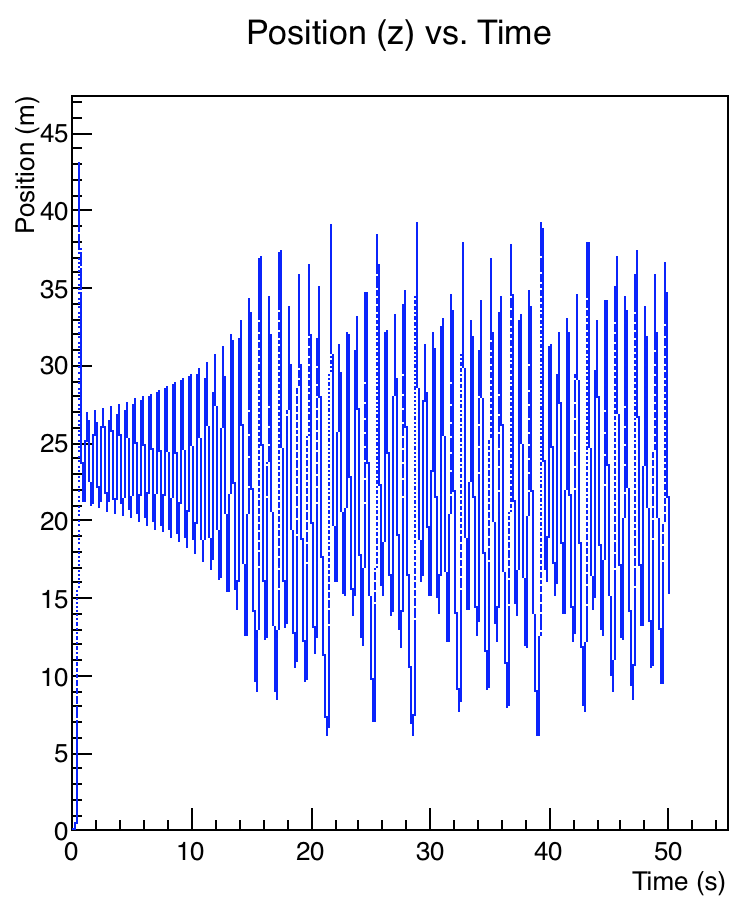
\includegraphics[scale=0.65]{fig-2.png}
	\end{center}
	\caption{The graph $z$ vs. $t$ after solving by the Euler method. This can be compared to figure 3.15 in the Giordano/Nakanishi textbook.}
\end{figure}

As a final note on my results, I found that the Lorenz model does indeed show considerable sensitivity to the initial conditions provided by the
user. The following graph shows the projection of two solutions, plotted on the same graph. Their number of points, value of $\Delta t$, and
parameters used were all identical. The only difference between the two solutions is the quantity of $\epsilon = 0.01$ added to the $x_0$
coordinate of the solution graphed in red. Despite this minor change in the initial conditions, the clear difference between the two graphs 
makes the system's sensitivity more visible.
\begin{figure}[h]
	\begin{center}
		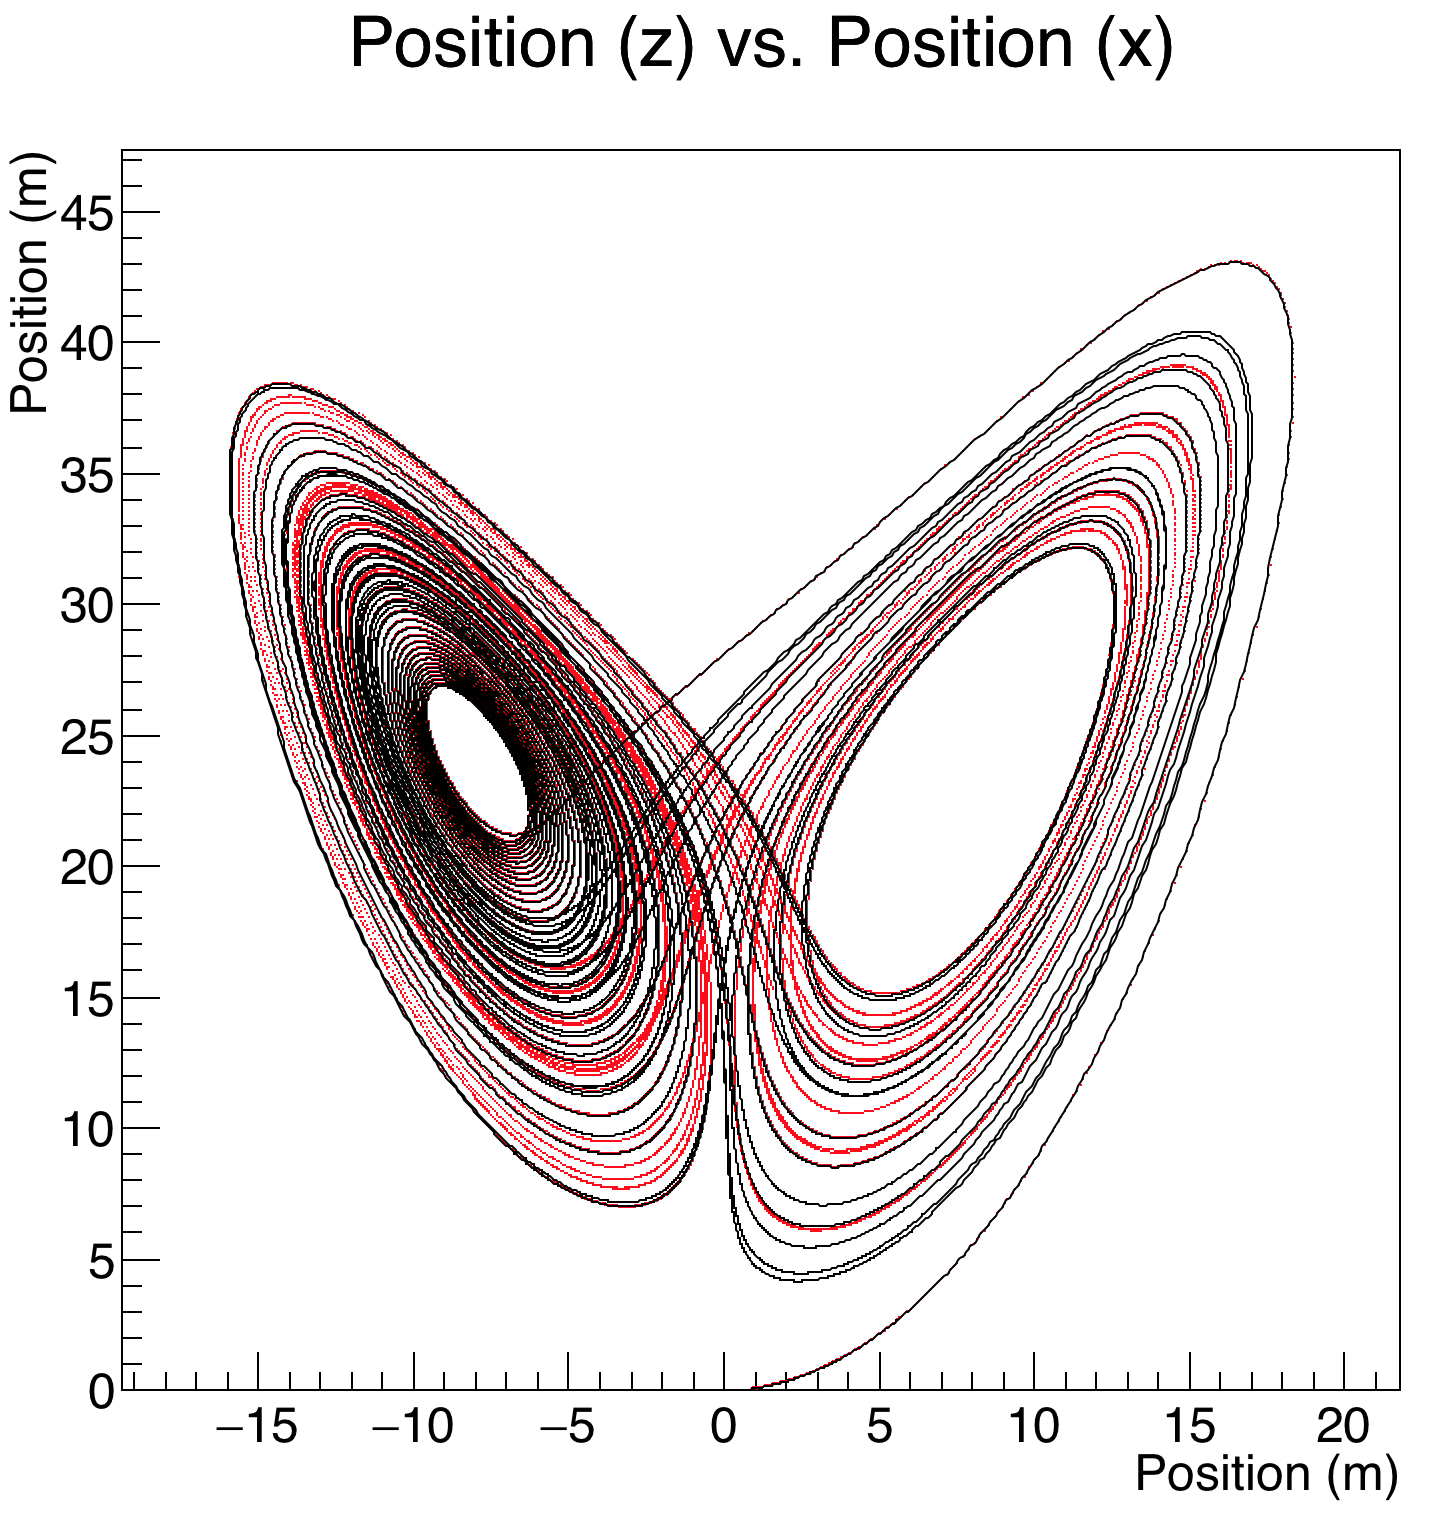
\includegraphics[scale=0.33]{fig-3.png}
	\end{center}
	\caption{Two graphs of the $x$-$z$ axis with an $\epsilon = 0.01$ difference in their initial $x$-coordinate.}
\end{figure}

Overall, my program appears to correctly solve the problem, but future versions might focus on attempting to correct its behavior for larger
(less precise) values of $\Delta t$. Alternatively, the textbook also mentions the Runge-Kutta method, which may be able to allow the user to
solve the differential equations with less precision. It would also be worthwhile to compare the algorithmic efficiency and error of the two
approaches. It could turn out, for instance, that the Euler method is actually better suited for this problem given its $O(N)$ time efficiency. 
Future versions might also focus on supporting larger values of $N$ and smaller values of $\Delta t$. I discuss this further in the next section.

\newpage
\section{Stability of the Numerical Method}
As mentioned in the previous sections, the Euler method provides an accurate solution to the Lorenz equations for sufficiently low values of 
$\Delta t$. I found that overall, the maximum precision still yielding accurate results is $\Delta t = 0.01$. The number of points to plot, $N$,
generally only affects the appearance of the graph, since graphs with too few points will tend to look sparse or incomplete (like in the image 
below). To counteract this, the solution might seem to be to add more points.

For example, when I ran my program with $N = 100,000$ and $\Delta t = 0.0001$, the graphs did not have enough points to exhibit chaos, as
demonstrated below. 
\begin{figure}[h]
	\begin{center}
		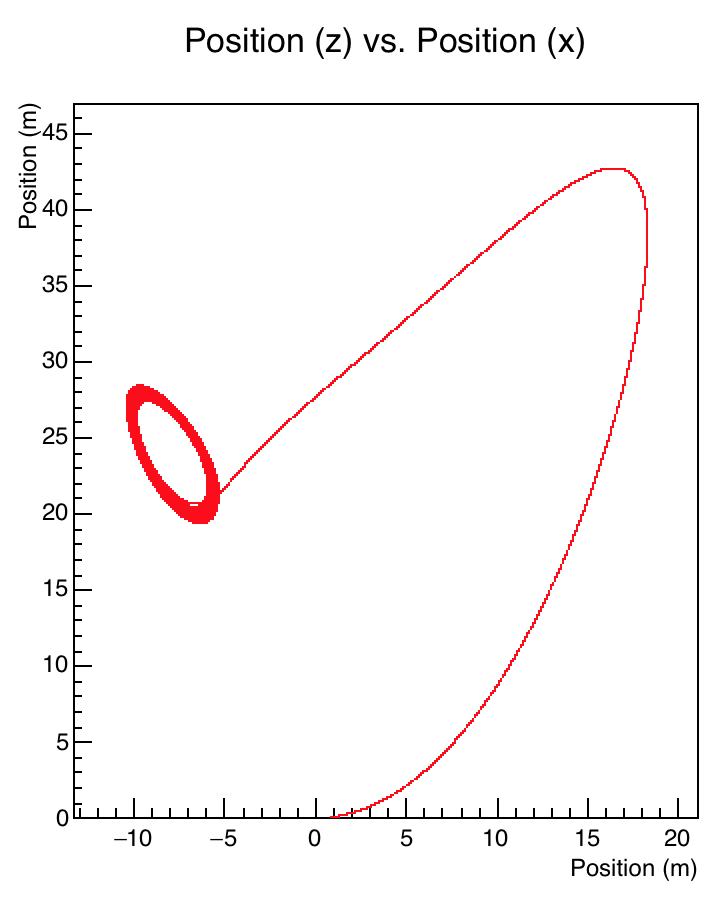
\includegraphics[scale=0.63]{fig-4.png}
	\end{center}
	\caption{The projection of the solution set onto the $x$-$z$ axis. While this should resemble figure 1, there were not enough points to
	exhibit chaotic behavior. While we can actually begin to see chaotic behavior for values of $N$ as large as $250,000$, this still does not
	lend us much insight into the system's overall behavior as we evolve the system further. If we go much past this value of $N$, we get a
	segmentation fault. }
\end{figure}

Yet, when I attempted to increase the number of points to $N = 1,000,000$ with the same precision, the execution terminated quickly with 
segmentation fault. My best guess is that this can be attributed to the operating system preventing the program from using more memory, rather
than error in the Euler method; arrays with $1,000,000$ elements are no doubt taxing on the system's memory. Instead, it might be better to use
a different data structure to store the arrays for $t$ and the $x$, $y$, and $z$ solutions. I would be interested to see whether or not using linked
lists would crash the program, since arrays are contiguous blocks of memory while linked lists are not.

Finally, altering the initial conditions and parameter values ends up having little impact on the correctness and accuracy of the Euler method. In
my implementation of the program, I detected if the user entered negative values of $\sigma$, $r$, and $b$ (which are all defined to be positive
in the book's discussion of the problem) and then set them to preset default values, so I was unable to investigate the potentially strange
behavior that may result from the three parameters assuming negative values. I did experiment with setting one, two, or three of the parameters
equal to zero and generally had uninteresting results. I found that this generally produced very uninteresting graphs (mostly linear and
exponential).

I also experimented with multiplying one or many of the parameters by constant factors, but generally did not find any interesting results here
either. In one of my executions of the program (using $N = 50,000$, $\Delta t = 0.001$, $\sigma = 5.0$, $b = 1.333$, $r = 12.50$, and 
$x_0 = 1.0$, $y_0 = z_0 = 0.0$), the $(x, y, z)$ solution appeared to converge to approximately $(-4, -4, 12)$, spiraling into the point as $t$ 
increased. Preserving the same values of $N$, $\Delta t$, and initial conditions, my execution of the program with each of the parameters
doubled matched closely with the original graphs seen in figures 1 and 2.

\end{document}  